%!TEX TS-program = pdflatex
\documentclass{article}
\usepackage[round]{natbib}
\usepackage{graphicx}
\usepackage{pifont,fancybox,multicol,palatcm}
\usepackage{caption}
\usepackage{float}
\usepackage{fancyhdr}
\usepackage{geometry}
\pagestyle{fancy} 
\geometry{margin=1.2in,top=1in,bottom=1in}
\usepackage{amsmath,amssymb}
\usepackage{bm}
\usepackage{textcomp}
\usepackage[usenames,dvipsnames]{color}
\usepackage[pdfmenubar=false,pdftex,pdfpagelabels=true,colorlinks=true,linkcolor=ISBABlue,citecolor=ISBABlue,urlcolor=DarkOrange]{hyperref}
\usepackage[export]{adjustbox}
\usepackage{soul}
\usepackage{wrapfig}
\usepackage{subcaption}
\usepackage{tabularx, booktabs}
%%%% Features this issue
\usepackage{pgfplots}
\usepackage{tikz}
\usepackage{url}
\usepackage{placeins}
%%%%




\graphicspath{{figures/}}

\usepackage{framed}
\makeatletter
\newenvironment{kframe}{%
 \def\at@end@of@kframe{}%
 \ifinner\ifhmode%
  \def\at@end@of@kframe{\end{minipage}}%
  \begin{minipage}{\columnwidth}%
 \fi\fi%
 \def\FrameCommand##1{\hskip\@totalleftmargin \hskip-\fboxsep
 \colorbox{shadecolor}{##1}\hskip-\fboxsep
     % There is no \\@totalrightmargin, so:
     \hskip-\linewidth \hskip-\@totalleftmargin \hskip\columnwidth}%
 \MakeFramed {\advance\hsize-\width
   \@totalleftmargin\z@ \linewidth\hsize
   \@setminipage}}%
 {\par\unskip\endMakeFramed%
 \at@end@of@kframe}
\makeatother

\parskip 1.5ex
\parindent 0em

\newcommand{\para}[1]{\vspace{.3em}\textbf{#1}\par}

\newcommand{\issue}{ISBA Bulletin, \textbf{32}(3), September 2025}
\newcommand{\blue}[1]{\textcolor{blue}{#1}}

\newcommand{\MyFilledBox}[1]{
\label{#1}
\vspace{1em}
\markright{\emph{#1}}{}
\hypertarget{#1}{}
\fcolorbox{White}{LightBlue}
{\begin{minipage}[t]{15.3cm}
\begin{center}

	\vspace{2.4mm}
	\subsection*{#1}

	\vspace{.3mm}
\end{center}
\end{minipage}}
\vspace{1mm}}

\newcommand{\MyFilledbox}[2]{
\hspace{-2.3mm}
\fcolorbox{White}{LightBlue}
{
\begin{minipage}[t]{#2}
	\begin{center}
	
		\textbf{\large #1}
	
	\end{center}
\end{minipage}}\\[2mm]}

\newcommand{\MyFancyBox}[3]{
\hspace{-4mm}
\fcolorbox{Black}{VeryLightBlue}{
\begin{minipage}[t]{#3}
	\MyFilledbox{#1}{#3}\\
	#2
\end{minipage}
}}

\newcommand{\MyFancyBoxWhite}[3]{
\hspace{-4mm}
\fcolorbox{Black}{White}{
\begin{minipage}[t]{#3}
	\MyFilledbox{#1}{#3}\\
	#2
\end{minipage}
}}

\renewcommand{\sectionmark}[1]{\markboth{#1}{}}

\definecolor{ISBABlue}{rgb}{0, .122, .388}
\definecolor{LightBlue}{rgb}{0.70, 0.75, 0.85}
\definecolor{VeryLightBlue}{rgb}{0.95,0.95,0.99}
\definecolor{DarkOrange}{rgb}{.9, 0.39, 0.0}

\fancyhead[L]{\issue}
\fancyhead[R]{}
\fancyfoot[C]{\thepage}
\fancyfoot[R]{\tt \href{https://www.bayesian.org}{www.bayesian.org}}

%---------- packages and commands for code blocks @software
\usepackage{mathtools}
\usepackage{fancyvrb}
\newcommand{\VerbBar}{|}
\newcommand{\VERB}{\Verb[commandchars=\\\{\}]}
\DefineVerbatimEnvironment{Highlighting}{Verbatim}{commandchars=\\\{\}}
% Add ',fontsize=\small' for more characters per line
\definecolor{shadecolor}{RGB}{248,248,248}
\newenvironment{Shaded}{\begin{snugshade}}{\end{snugshade}}
\newcommand{\AlertTok}[1]{\textcolor[rgb]{0.94,0.16,0.16}{#1}}
\newcommand{\AnnotationTok}[1]{\textcolor[rgb]{0.56,0.35,0.01}{\textbf{\textit{#1}}}}
\newcommand{\AttributeTok}[1]{\textcolor[rgb]{0.13,0.29,0.53}{#1}}
\newcommand{\BaseNTok}[1]{\textcolor[rgb]{0.00,0.00,0.81}{#1}}
\newcommand{\BuiltInTok}[1]{#1}
\newcommand{\CharTok}[1]{\textcolor[rgb]{0.31,0.60,0.02}{#1}}
\newcommand{\CommentTok}[1]{\textcolor[rgb]{0.56,0.35,0.01}{\textit{#1}}}
\newcommand{\CommentVarTok}[1]{\textcolor[rgb]{0.56,0.35,0.01}{\textbf{\textit{#1}}}}
\newcommand{\ConstantTok}[1]{\textcolor[rgb]{0.56,0.35,0.01}{#1}}
\newcommand{\ControlFlowTok}[1]{\textcolor[rgb]{0.13,0.29,0.53}{\textbf{#1}}}
\newcommand{\DataTypeTok}[1]{\textcolor[rgb]{0.13,0.29,0.53}{#1}}
\newcommand{\DecValTok}[1]{\textcolor[rgb]{0.00,0.00,0.81}{#1}}
\newcommand{\DocumentationTok}[1]{\textcolor[rgb]{0.56,0.35,0.01}{\textbf{\textit{#1}}}}
\newcommand{\ErrorTok}[1]{\textcolor[rgb]{0.64,0.00,0.00}{\textbf{#1}}}
\newcommand{\ExtensionTok}[1]{#1}
\newcommand{\FloatTok}[1]{\textcolor[rgb]{0.00,0.00,0.81}{#1}}
\newcommand{\FunctionTok}[1]{\textcolor[rgb]{0.13,0.29,0.53}{\textbf{#1}}}
\newcommand{\ImportTok}[1]{#1}
\newcommand{\InformationTok}[1]{\textcolor[rgb]{0.56,0.35,0.01}{\textbf{\textit{#1}}}}
\newcommand{\KeywordTok}[1]{\textcolor[rgb]{0.13,0.29,0.53}{\textbf{#1}}}
\newcommand{\NormalTok}[1]{#1}
\newcommand{\OperatorTok}[1]{\textcolor[rgb]{0.81,0.36,0.00}{\textbf{#1}}}
\newcommand{\OtherTok}[1]{\textcolor[rgb]{0.56,0.35,0.01}{#1}}
\newcommand{\PreprocessorTok}[1]{\textcolor[rgb]{0.56,0.35,0.01}{\textit{#1}}}
\newcommand{\RegionMarkerTok}[1]{#1}
\newcommand{\SpecialCharTok}[1]{\textcolor[rgb]{0.81,0.36,0.00}{\textbf{#1}}}
\newcommand{\SpecialStringTok}[1]{\textcolor[rgb]{0.31,0.60,0.02}{#1}}
\newcommand{\StringTok}[1]{\textcolor[rgb]{0.31,0.60,0.02}{#1}}
\newcommand{\VariableTok}[1]{\textcolor[rgb]{0.00,0.00,0.00}{#1}}
\newcommand{\VerbatimStringTok}[1]{\textcolor[rgb]{0.31,0.60,0.02}{#1}}
\newcommand{\WarningTok}[1]{\textcolor[rgb]{0.56,0.35,0.01}{\textbf{\textit{#1}}}}
%----------

\begin{document}
\hypertarget{TOP}{}
\thispagestyle{empty}
{\hfill \sc September 2025}

\vspace*{-.7em}
{\hfill \sc Vol.\ 32 No.\ 3}

\vspace*{-1.5em}
\begin{center}

\includegraphics[width=7cm]{isbalogo}
\end{center}
\fcolorbox{Black}{LightBlue}
{
\begin{minipage}[t]{15.1cm}
	\begin{center}	  
		\vspace{.5em}
%		\includegraphics[width=5cm]{isbalogotrans}\\[2em]
		\textbf{\Huge{ \sc{The \hspace{.1mm} ISBA\hspace{3mm} Bulletin}}}\\[2mm]
%		 		 {\sc Vol.\ 28 No.\ 1 \hfill  March 2021}\\[1pc] 				 
		 		 {\sc {\large Official bulletin of the International Society for Bayesian Analysis}}
		 		 \vspace{.5em}
	\end{center}
\end{minipage}
}


\clearpage

%%%%%%%%%%%%%%%%%%%%%%%%%%%%%%%%%%%%%%%%%%%%%%%

\newcommand{\citebi}{\cite}
\newcommand{\citein}{\cite}
\newcommand*{\subtitleproc}[1]{}
\newcommand*{\chapb}{}
\providecommand{\doi}[1]{}
\renewcommand{\doi}[1]{\href{https://doi.org/#1}{doi:#1}}
\newcommand*{\osfdoi}{doi}
\newcommand*{\amp}{\&}
%% Probability macros
\renewcommand*{\P}{\mathrm{P}}%probability
\renewcommand*{\|}[1][]{\nonscript\:#1\vert\nonscript\:\mathopen{}}
\newcommand*{\mo}[1][=]{\mathclose{}\mathord{\nonscript\mkern0.5mu#1\nonscript\mkern0.5mu}\mathopen{}}
\newcommand*{\yF}{F}
\newcommand*{\yf}{f}
\newcommand*{\di}{\mathop{}\!\mathrm{d}}
%%
\newcommand*{\HV}{\mathrm{HV}}
\newcommand*{\GDS}{\mathrm{GDS}}
\newcommand*{\cAD}{\mathrm{cAD}}
\newcommand*{\yy}{\mathrm{Y}}
\newcommand*{\yn}{\mathrm{N}}


\MyFilledBox{SOFTWARE HIGHLIGHT}
\begin{center}
{\large Luca\enspace Porta Mana} \\
{\tt \href{mailto:pgl@portamana.org}{pgl@portamana.org}}


\Large
\textsc{inferno\\
INFERence in R with Bayesian NOnparametrics}
\end{center}

\section{Population inference and Bayesian nonparametrics}
\label{sec:popinference}

A very important kind of inference in research fields such as medicine is \emph{population inference}, often also called ``density inference'' or ``density regression''. Its general goal is to infer the frequency distribution of some variates in a population. This is different, for instance, from \emph{functional regression}, where the goal is to infer the functional relationship -- assumed to exist -- between a set of predictor variates and a target or ``predictand'' variate. In population inference the existence of a functional relation cannot be assumed. In fact there may not even be a clear distinction between predictor and predictand variates. A typical goal is the inference of frequency distributions within particular sub-populations or sub-groups, thus all kinds of conditional probabilities are required. A clinician may be interested in the statistics and probability of a medical condition given a symptom, but also that of a symptom given a medical condition; and maybe only within subjects of a given sex or age. De~Finetti's theorem \citep[see e.g.][\S\S\,4.2, 4.3, 4.6]{bernardoetal1994_r2000} lies at the heart of population-inference methods; a particularly brilliant discussion is given by Lindley \& Novick \citeyearpar{lindleyetal1981}.

Sadly many researchers still approach population-inference problems by means of $p$-values or other frequentist practices, which only give limited, coarse, and not seldom misleading results about a population's frequency distribution. Some researchers adopt Bayesian methods but limit themselves to \emph{parametric} ones, which make very restrictive and possibly unrealistic assumptions about the population's distribution; as opposed to \emph{nonparametric} ones, which don't.

Until a couple decades ago the use of parametric methods, and maybe even of frequentist practices, was somehow justified by pragmatic reasons. Better methods were computationally too costly or unfeasible. Population-inference problems were low-dimensional; one could \emph{visually} check whether the assumptions were appropriate to the problem and the results reasonable. Today the reasons cannot be earnestly be given, however. Bayesian nonparametric methods have become computationally feasible for many kinds of population inference. And many population-inference problems today involve tens, hundreds, or thousands of variates of different kinds; being so high-dimensional, it is impossible to visually check whether frequentist practices or parametric assumptions are acceptable, or by how much they err. Results may therefore be affected by large errors \citep{draper1995}, whose existence is often not even reported.

One reason can still be given today for the avoidance of Bayesian nonparametric methods for population inferences: \emph{lack of user-friendly software}. Clinicians who'd be curious to try out a Bayesian nonparametric analysis of their studies simply can't: that would require the study of Markov-chain Monte Carlo techniques, of programming languages to implement the latter, and of a plethora of debated practices to ``assess convergence''. Most clinicians don't have time to learn all this even if they wanted to. Available packages for Bayesian nonparametrics are not quite suited to population inference. Some focus on functional regression, which as discussed above is not an appropriate assumption. Some make an a priori distinction between predictor and predictand variates, limiting the range of useful inferences. Most still require non-statistical technical expertise.

\medskip

The R-package \textbf{inferno}\footnote{\url{https://pglpm.github.io/inferno/}} was built to try to remedy the lack of this kind of software.

\section{Use and features}
\label{sec:features}

(In the following, for brevity, the term `probability' will also stand for `probability density' depending on nature of the quantities involved; similarly for `frequency'.)

The application of the package is simple. The user provides a sample of variates $D$ from a population, for instance the age, sex, symptom, disease, and kind of treatment of a number of patients. Thereafter, the user can calculate any of the following:
\begin{itemize}
\item For a new unit of the population, say a new patient, the conditional probability for the values of \emph{any} set of variates $X \mo x, Y \mo y, \dotso$ given \emph{any} other set $Z \mo z, W \mo w, \dotso$:
  \begin{equation}\label{eq:prob_var}
    \P(X \mo x, Y \mo y, \dotso \|Z \mo z, W \mo w, \dotso , D)
  \end{equation}
  Such a probability could for instance be used in medical decision making \citep{soxetal1988_r2024,huninketal2001_r2014}. The conditional could also be empty.

\item The probability distribution for the conditional \emph{frequencies}, in the whole unsampled population, of the values of any set of variates given any other set. If we denote by $\yF$ the frequency and by $\yf$ a specific value,
  \begin{equation}\label{eq:prob_freq}
    \P\bigl[ \yF(X \mo x, \dotso \|Z \mo z, \dotso) = \yf \|[\big] D\bigr]
    \ .
  \end{equation}
This probability distribution is represented by Monte Carlo samples drawn from it.

\item The mutual information \citep[Ch.~8]{mackay1995_r2005} between any two sets of quantities.
\end{itemize}

Probabilities~\eqref{eq:prob_var} and~\eqref{eq:prob_freq} are connected by a variant of de~Finetti's theorem:
\begin{equation}
  \label{eq:definetti1}
  \P(X \mo x, \dotso \|Z \mo z, \dotso , D)  =
  \int \yf \,
  \P\bigl[ \yF(X \mo x, \dotso \|Z \mo z, \dotso) = \yf \|[\big] D\bigr]
  \,\di\yf
\end{equation}

In a manner of speaking, the probability distribution~\eqref{eq:prob_freq} expresses how much the probability value~\eqref{eq:prob_var} could change, if it were updated by sampling the whole population. It expresses the uncertainty in the statistical results owing to finite sample size.


\begin{figure}[t]\caption{}\label{fig:distr}
  \centering
  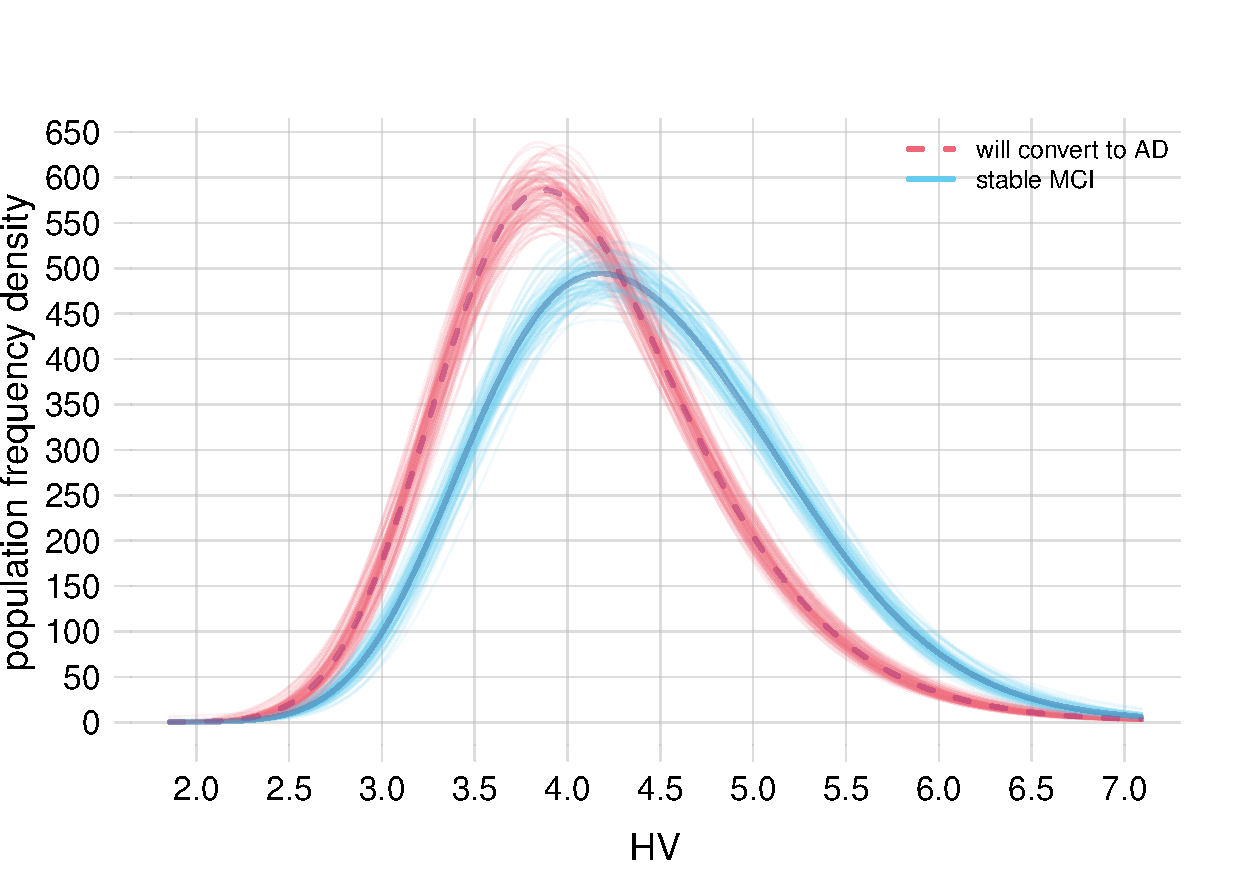
\includegraphics[width=0.49\linewidth]{figures/population_distr_HV.pdf}\hfill%
  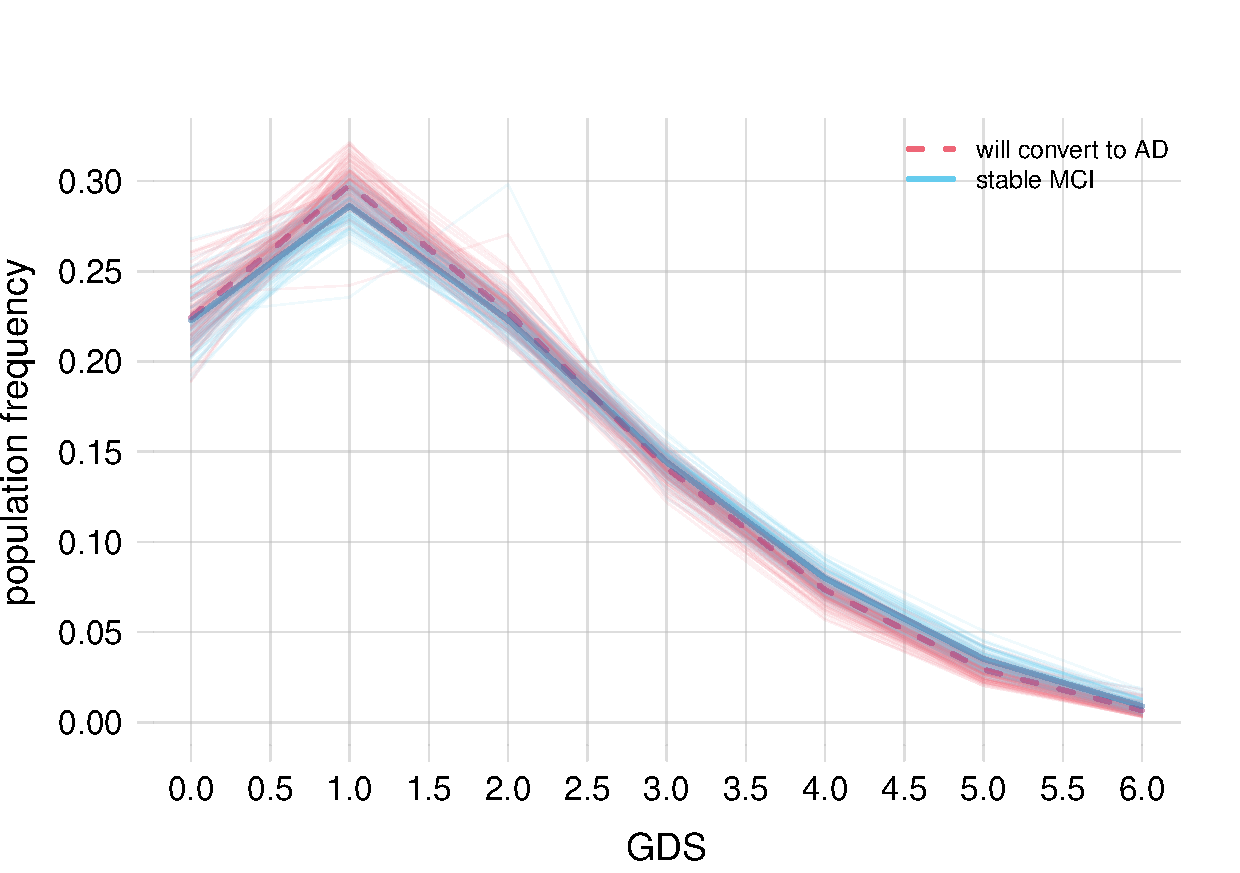
\includegraphics[width=0.49\linewidth]{figures/population_distr_GDS.pdf}
\end{figure}
The package allows the user to visualize the probabilities above when just one ``predictand'' and one predictor variates are involved.
Figure~\ref{fig:distr} shows two examples from a study \citep{portamanaetal2023b} about conversion from Mild Cognitive Impairment (MCI) to Alzheimer's Disease (AD); they can be used to further illustrate the probability distributions discussed above.

In the plot on the left, the predictand variate is hippocampal volume ($\HV$); the predictor is the binary, yes/no variate `will convert to AD' ($\cAD$). The solid blue thick line and dashed red thick line are the conditional probability distributions (omitting the data dependence)
\begin{equation*}
  \P( \HV \| \cAD \mo \yn)\ ,\qquad
  \P( \HV \| \cAD \mo \yy) \ .
\end{equation*}
The cloud of blue thinner lines that surrounds the first distribution above  represents the probability distribution of possible frequency distributions
\begin{equation*}
  \P\bigl[ \yF(\HV \| \cAD \mo \yn)\bigr]
\end{equation*}
each thin line is a sample from such distribution.

Looking at this plot, a clinician can immediately see that the frequency distribution of hyppocampal volume is clearly different in the sub-populations of patients that will convert to Alzheimer's and those who won't. Such a difference is almost certain even considering the uncertainty from the finite sample size.

The plot on the right is analogous but for the predictand variate `geriatric depression scale' ($\GDS$) in stead of hippocampal volume. In this case the two conditional frequency distributions cannot be distinguished within the finite-sample uncertainty.

It must be remarked that it is exactly this kind of differences and uncertainties that clinical researchers often try to clumsily capture by using $p$-values. Several practitioners expressed relief and even awe at the possibility of visualizing the estimates of different sub-population statistics and even the uncertainties they carry because of finite sample size.

The quick analysis above was purely qualitative, but concrete numbers, such as quantiles and expected values, can be given instead. This becomes necessary when many variates are considered jointly and visualization is impossible. In such high-dimensional cases the package allows the user to compute any kind of distance between two frequency distributions (such as Hellinger or Kantorovich or Shannon-Jansen distance, or relative entropy) as well as its credibility intervals. The computation of the mutual information between any two sets of variates gives moreover a quantitative measure of their association that does not depend on assumptions such as linearity or gaussianity.

\medskip

\begin{figure}[t]\caption{}\label{fig:distr_inv}
  \centering
  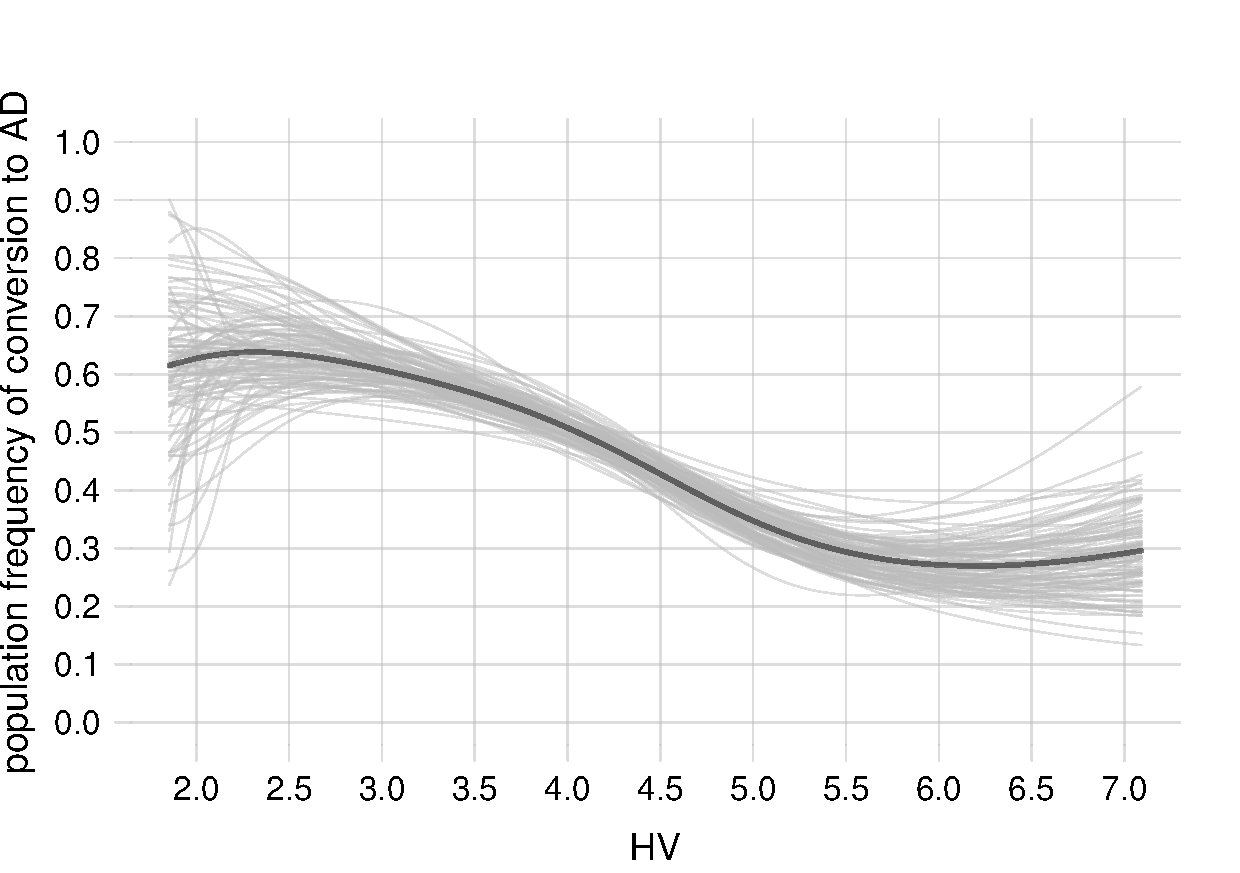
\includegraphics[width=0.49\linewidth]{figures/prob_conversion_HV.pdf}\hfill%
  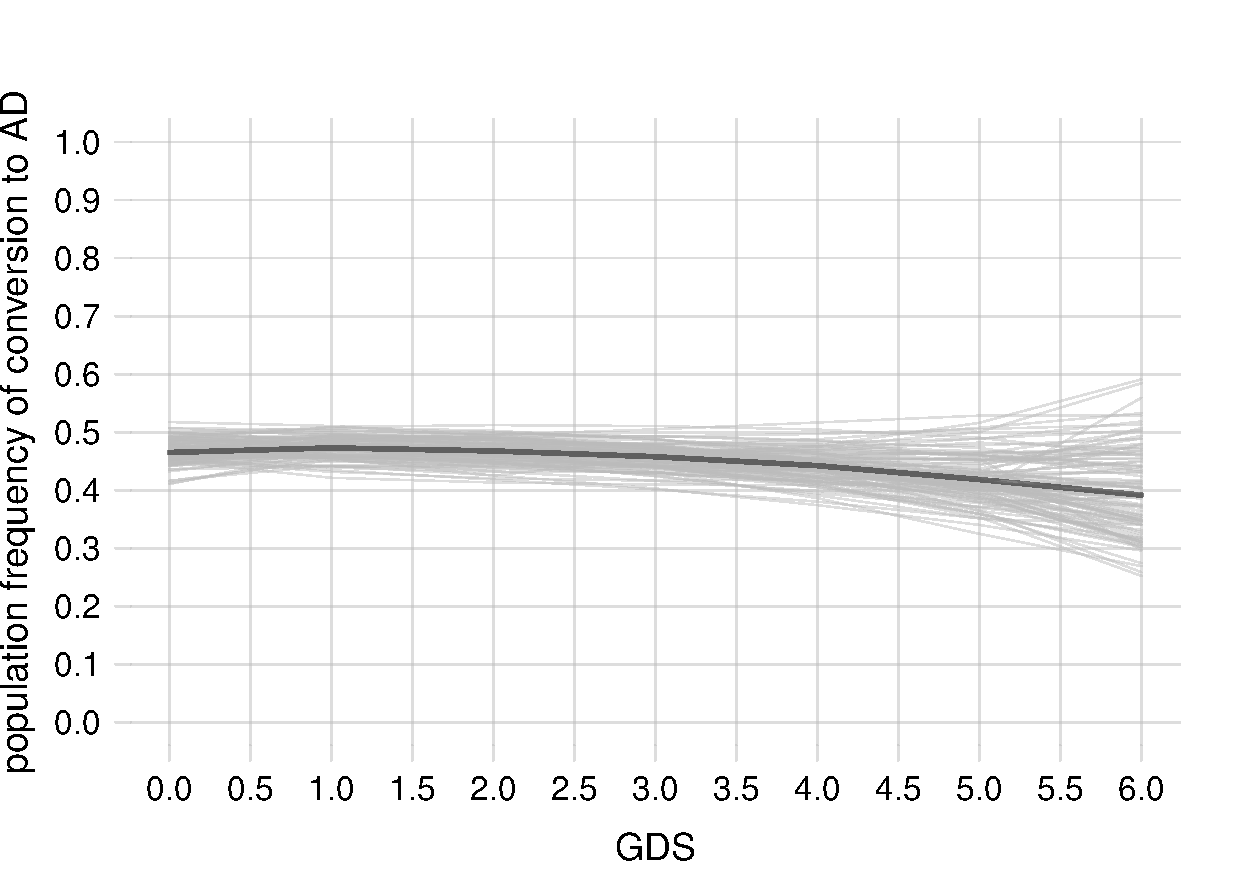
\includegraphics[width=0.49\linewidth]{figures/prob_conversion_GDS.pdf}
\end{figure}
The ability to swap the ``predictor'' and ``predictand'' roles of any variates is illustrated in the plots of fig.~\ref{fig:distr_inv}, which parallel those of fig.~\ref{fig:distr}. The thicker lines show the probabilities
\begin{equation*}
    \P( \cAD \mo \yy \| HV)\ ,\qquad
  \P( \cAD \mo \yy \| \HV)
\end{equation*}
for various values of the $\HV$ variate, which becomes a predictor in this case. The clouds of thinner lines are samples of the corresponding probability distributions of the frequency distributions. On the plot on the left, for instance, we see that among individuals from this population having hippocampal volume around $5.0$, between 30\% and 40\% will convert to Alzheimer's. Among those with volume around $2.0$, we can only say that between roughly 45\% and 80\% will convert; in this case the finite-sample size (few samples with this $\HV$ value) leads to a much larger uncertainty of the frequency estimates.

\medskip

The \textbf{inferno} package can work with any combination of continuous, discrete ordinal, discrete nominal, and binary variates. Continuous variates can also be defined in bounded intervals, and can also have boundary values capable of finite probability mass, as it may happen with censoring. The package cannot handle variates with complex topology, such as images, or periodic variates.

\section{Nonparametric representation}
\label{sec:representation}

In Bayesian nonparametric population inference the posterior probability distribution is over the set of all possible frequency distributions. The mathematical representation of this set is therefore crucial. The package uses the ingenious representation of a distribution as a mixture of product kernels introduced by Dunson \& Bhattacharya \citeyear{dunsonetal2011}. For instance, for variates $X$ and $Y$ the frequency distribution is written as
\begin{equation}
  \label{eq:mixture_kernel}
  \yF(X, Y) = \sum_{i} w_{i}\, K_{X}(X \| \xi_{i})\, K_{Y}(Y \| \upsilon_{i})
\end{equation}
where $w_{i}$ are positive and normalized weights, $K_{X}$ is a distribution for variate $X$ depending on parameters $\xi_{i}$, and similarly for $K_{Y}$. The product is easily generalized to any number of variates. In principle the sum should be countably infinite, but as discussed in Ishwaran \& Zarepour \citeyear{ishwaranetal2002b,ishwaranetal2002c} and in Dunson \& Bhattacharya \citeyear{dunsonetal2011}, it is possible to truncate it to a finite number of values if an appropriate prior distribution is used for the weights $w_{i}$. Thus a frequency distribution $\yF$ is effectively represented -- non-uniquely -- by a large but finite set of parameters $(w_{i}, \xi_{i}, \upsilon_{i})$.


The above representation by products of individual kernels has been somewhat deprecated in more recent works \citep[e.g.][]{wadeetal2014,wadeetal2014b} which, however, consider inference problems where variates have clear predictor or predictand roles. As previously discussed, in many research fields such roles have no clear a-priori division and are quite dynamic. A representation that easily allow to swap the two role of variates, without overemphasizing either, is therefore most appropriate. The representation~\eqref{eq:mixture_kernel} leads to very simple and symmetric analytical expressions for the conditional of $X$ given $Y$ and vice versa, as well as any marginal:
\begin{equation*}
  \begin{gathered}
    \yF(X \| Y) = \sum_{i}
    \frac{w_{i}}{\sum_{j} w_{j}K_{Y}(Y \| \upsilon_{j})}\, K_{X}(X \| \xi_{i})\, K_{Y}(Y \| \upsilon_{i})
    \\
    \yF(Y \| X) = \sum_{i}
    \frac{w_{i}}{\sum_{j} w_{j}K_{X}(X \| \xi_{j})}\, K_{Y}(Y \| \upsilon_{i})\, K_{X}(X \| \xi_{i})
    \\
    \yF(X) = \sum_{i}
    w_{i}\, K_{X}(X \| \xi_{i}) \ .
  \end{gathered}
\end{equation*}



This posterior is represented by samples of such distributions, obtained by Markov-chain Monte Carlo.




[bayes base rate]


\citep{walker2010}

\bibliographystyle{abbrvnat}
\bibliography{../manual/portamanabib.bib}

\end{document}
, that is, the inference of a functional relationship -- assumed to exist -- between a set of predictor variates and a target or ``predictand'' variate. These packages are not appropriate to \emph{population inference}, where no functional relationships exist a priori, and where often there is no a priori division between predictor and predictand variates. In clinical studies one may be interested in calculating the probability of an effect or symptom given a condition, and of a condition given an effect or symptom.
